\chapter{Validation in liquid jet in crossflow}
	\label{ch6:jicf_lgs_simulations}


%Describe here all our results from the lagrangian simulations:
%
%\begin{itemize}
%
%	\item Effects of applying full workflow: w/wo ALM, w/wo secondary atomization ...
%	
%	\item Mesh convergence study: specify it
%	
%	\item Validation with experiments
%	
%	\item Mass conservation issues: lagrangian tracking, etc. 
%	
%
%\end{itemize}


\section{Introduction}

This chapter presents results from lagrangian simulations performed with the SLI models described in Chapter \ref{ch4:sli_development}. The test case used is the academic JICF of \citeColor[becker_breakup_2002], for which resolved simulations of the atomization process were detailed in Chapter \ref{ch5:jicf_resolved_simulations}. Data for these computations are used to build the injectors in order to run dispersed phase simulations in the same configuration, which are shown to be less computationally expensive than the resolved ones. \hl{...}


\section{Computational setup}

The geometry replicating the experimental test bench is the same than the one used for the resolved simulations, depicted in Figure \ref{fig:numerical_setup_maquette_JICF_DLR}. The operating points simulated are the ones from Table \ref{tab:jicf_operating_conditions}. Regarding the mesh employed, it was shown in $\S$\ref{sec:ch5_initial_conditions} that an element size of $\Delta x = 0.5$ mm allows to transport the estimated turbulence in these cases. Nevertheless, the simulations from Chapter \ref{ch5:jicf_resolved_simulations} use a mesh with this cell size only inside the plenum upstream and around the injector, while downstream the injector the mesh size is enlarged since there is no liquid at this region. This mesh was shown in Figure \ref{fig:jicf_dlr_mesh}. In the lagrangian simulations performed in this chapter, injection is performed at the sampling planes downstream the injector \hl{shown in Chapter }\ref{ch5:jicf_resolved_simulations}, and the region of interest extends up to a location at $x = 80$ mm downstream the injector since this is where validation with the experimental results of \citeColor[becker_breakup_2002] can be performed. Therefore, lagrangian simulations use a baseline cell size of $\Delta x = 0.5$ mm in the plenum from the gaseous inlet up to $x = 85$ mm downstream the injector. In this way, turbulence can be transported from the gaseous inlet  up to the experimental validation plane. \hl{The mesh used, shown in Figure} \ref{fig:jicf_dlr_mesh_LGS}, is composed of \textbf{XX} elements, being therefore larger than the baseline mesh employed for the resolved simulations. However, in the dispersed phase simulations there is no Adaptive Mesh Refinement being performed, and therefore the number of mesh elements stays constant in all simulations.


\begin{figure}[h!]
	\centering
	\includeinkscape[inkscapelatex=true,scale=0.8]{./part2_developments/figures_ch6_lagrangian_JICF/jicf_mesh_LGS}
	\caption{Mesh employed for LGS simulations. \hl{CHANGE WHEN READY}}
	\label{fig:jicf_dlr_mesh_LGS}
\end{figure}

%\section{Evaporation phenomena}
%
%\textbf{Note: this analysis could perfectly be in the previous chapter}.
%
%As indicated in Table \ref{tab:jicf_operating_conditions}, the temperatures of both liquid kerosene and gaseous air are low (290 and 288 K respectively) and there is not direct evaporation of fuel. Nevertheless, some evaporation can occur at ambient temperature if the vapour pressure of the liquid is lower than the ambient pressure. In the experiments, the ambient pressure is $p_g = 6$ bar, while the vapour pressure of kerosene at $288$ K is $p_{vap} = 0.003$ bar \citepColor[shepherd_flash_2000]. Therefore, evaporation might be possible.
%
%It is tested that ... Two characteristic times are used in the low We case (since the lowest velocity is found there, and the droplets take more time to reach the validation plane at 80 mm)/
%
%\begin{itemize}
%
%	\item The time that a droplet takes to reach the plane x = 80 mm. From the SPS results in $\S$\textbf{??} (or Table \textbf{??}), the first droplets at x = 10 mm are obtained at $t_{resolv} = 0.3$ ms after injection. Then, the first droplets injected at this location in the lagrangian simulations reach the validation plane after $t_\mathrm{lagr} = $ ms. Hence, a characteristic time defined as the :
%	
%	\begin{equation}
%	\tau_{validation} = t_{resolv}  + t_\mathrm{lagr}
%	\end{equation}
%	
%	\item Evaporation time rate is used by means of the $d^2$ law. This law that the square of the droplet's diameter diminishes linearly with time:
%	
%	\begin{equation}
%	\label{eq:d2_law}
%	d^2 \left( \right) = d_0^2 - K t
%	\end{equation}
%	
%	
%	where $K$ is the evaporation rate and $d_0$ the initial diameter of the droplet. The value K ... (see 2006 Ghassemi).
%	
%	
%	\text{NAH}. The evolution in diameter after a given time $t$ can then be obtained as:
%	
%	\begin{equation}
%	\Delta d^2 = d_0^2 - d^2 \left( \right) = K t
%	\end{equation}
%	
%
%\end{itemize}

\section{Obtention of initial conditions with ALM}

Prior to liquid injection, it is necessary to establish an initial solution for the gaseous phase as done for the resolved simulations. The difference with respect to the resolved simulations is that in this case, the initial solutions needs to consider the ALM since the dense core blockage effect needs to be modelled in the dispersed phase simulations. All the details of the model were addressed in $\S$\ref{sec:ch4_dense_core_modelling}. In this section, firstly results from the resolved simulations are employed as input parameters to feed the ALM model. Secondly, gaseous simulations are performed with the ALM to obtain initial solutions. The resulting gaseous fields are compared to the ones of the resolved simulations to check the accuracy of the proposed ALM.

\subsection{Setup of actuator model}

The model parameters for ALM were described in Table \ref{tab:alm_parameters}. For the two operating points simulated, the corresponding input parameters are summarized in Table \ref{tab:jicf_lgs_ALM_parameters}. The points $x_b$, $z_b$ and $c_L$ are obtained from the mean values of Figure \ref{fig:dense_core_mean_parameters_scatterplots} for the fine simulations (note that $c_L$ is equivalent to the resolved dense core width $w$); $c_0$ is equal to the injector diameter; $N_p$ has been set to 20 as default, but it has been checked not to have an effect on the results; and the force $\textbf{F}_\mathrm{DC}$ is obtained as explained in $\S$\ref{ch5:subsec_defining_pressure_differences}.

\begin{table}[!h]
\centering
\caption{Parameters of an actuator representing the dense core}
\begin{tabular}{cccc}
\thickhline
\textbf{Parameter} & \textbf{Units} & \textbf{Low Weber} &  \textbf{High Weber} \\
\thickhline
$x_b$ & mm & & \\
$z_b$ & mm & & \\
$c_0$ & mm & 0.45 & 0.45 \\
$c_L$ & mm & & \\
$N_p$ & - & 20 & 20 \\
$| \textbf{F}_\mathrm{DC} |$ & N &  & \\
%$\Delta p$ & Pa &  & \\
\thickhline
\end{tabular}
\label{tab:jicf_lgs_ALM_parameters}
\end{table}

An example of an actuator representing the dense core in gaseous simulations \hl{can be seen in Figure }. As observed, it is graphically represented as a cylinder with the initial point located in the injection nozzle exit and final point in the breakup location of the resolved dense core estimated from the resolved simulations. The actuator points (not shown in the figure) are located uniformly along the central line of the cylinder. The discrete forces applied to each point are then mollified in the neighbouring cells in order to avoid flow singularities.

\subsection{Comparison between resolved and ALM gaseous fields}

The perturbed gaseous fields created by the presence of the dense core in the \hl{resolved simulations were discussed in $\S$}\ref{ch5:subsec_turbulent_structures_in_gaseous_field}. In the same fashion, equivalent postprocessings can be performed for the gaseous flow field 

A quantitative assessment of the actuator blockage effect can be performed by looking at the mean velocity distribution along the lines \textbf{XX} shown in Figure \ref{XX}. Equivalent data was obtained for the resolved simulations in \hl{\textbf{$\S$XX}}, which is also shown in the same Figure for comparison ...

\section{Relation between volume and mixture fractions}

So we can relate $\overline{\alpha}$ field with the mixture fraction somehow, this will be interesting for people doing combustion. I have developed the following relation between mixture fraction $Z$ and volume fraction $\alpha$ (need to check it properly):

\begin{equation}
Z = \frac{m_l}{m_l + m_g} = \frac{V_l \rho_l}{V_l \rho_l + V_g \rho_g} = \frac{1}{1 + \frac{V_g}{V_l} \frac{\rho_g}{\rho_l}} = \frac{1}{1 + \frac{\rho_g}{\rho_l} \frac{1 - \alpha}{\alpha}}
\end{equation}


We can also make a link to heat relase, for the interest of combustion studies.

\section{Experimental results}

In the configuration of \textbf{ref:2002-becker}, there are experimental results we can use for comparison at x = 80 mm. These include maps of SMD and flux (see Figure \textbf{XX}). We can also validate with quantitative results obtained by integrating the flux and SMD along the $y$ direction:

\begin{equation}
\langle q_l \left( z \right) \rangle = \frac{1}{L_y} \int_0^{L_y} q_l \left( y, z \right) dy ~~~~; ~~~~ \langle SMD \left( z \right) \rangle = \frac{1}{L_y \langle q_l \left( z \right) \rangle} \int_0^{L_y} q_l \left( y, z \right) SMD \left( y, z \right) dy
\end{equation}

In the same fashion, the results can be integrated along the $z$ direction to yield dependence with the $z$ axis:

\begin{equation}
\langle q_l \left( y \right) \rangle = \frac{1}{L_z} \int_0^{L_z} q_l \left( y, z \right) dz ~~~~; ~~~~ \langle SMD \left( y \right) \rangle = \frac{1}{L_z \langle q_l \left( z \right) \rangle} \int_0^{L_z} q_l \left( y, z \right) SMD \left( y, z \right) dz
\end{equation}


\section{Models sensitivity}

ALSO: effect of one and two-way coupling !! Ver articulos 2010, 2011 Li 

\subsection{Effect of injection conditions}

\subsection{Effect of secondary atomization model}

\subsection{Effect of dense core blockage effect model}

\section{Results}

\subsection{Mesh convergence study}

\subsection{Validation with experiments (quantitative/qualitative)}

\subsection{Trajectories}

In order to illustrate the lagrangian trajectories and the continuity with respect to the resolved jets, a volume fraction field can be defined in the lagrangian simulations:

\begin{equation}
\alpha_l \left( \textbf{x}, t \right) = \frac{V_l \left( \textbf{x}, t \right)}{V_{el}}
\end{equation}

where $V_{el}$ is the volume of the element in the eulerian mesh grid. Therefore, the volume fraction is a magnitude defined in the main eulerian grid. Since the dispersed phase is not directly represented in this grid but by lagrangian particles, $V_l \left( \textbf{x}, t \right)$ is calculated by interpolating the volume of the particles located within each element at each iteration.

\subsection{Frequential analysis}

Several probes have been located in the outer part of the jet to see the spectra. See Figures \ref{fig:probes_dx10m} and \ref{fig:probes_dx20m} for volume fraction probes, and Figure \ref{fig:probes_U_planey0} for determining velocity spectra at plane y = 0. These are available at pilotage 30-04-2021.

Para velocidades: OJITO con la probe 18 !

\begin{figure}[h!]
	\centering
	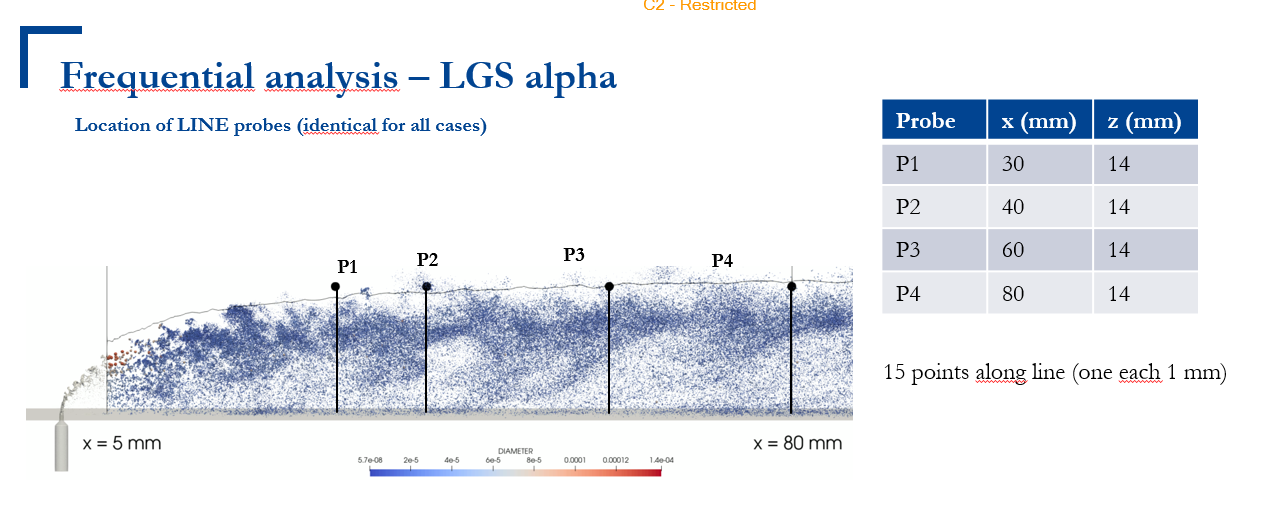
\includegraphics[scale=0.7]{./part2_developments/figures_ch6_lagrangian_JICF/probes_vol_frac}
	\caption{Probes for $\alpha$ frequential analysis for volume fraction}
	\label{fig:probes_dx10m}
\end{figure}


\begin{figure}[h!]
	\centering
	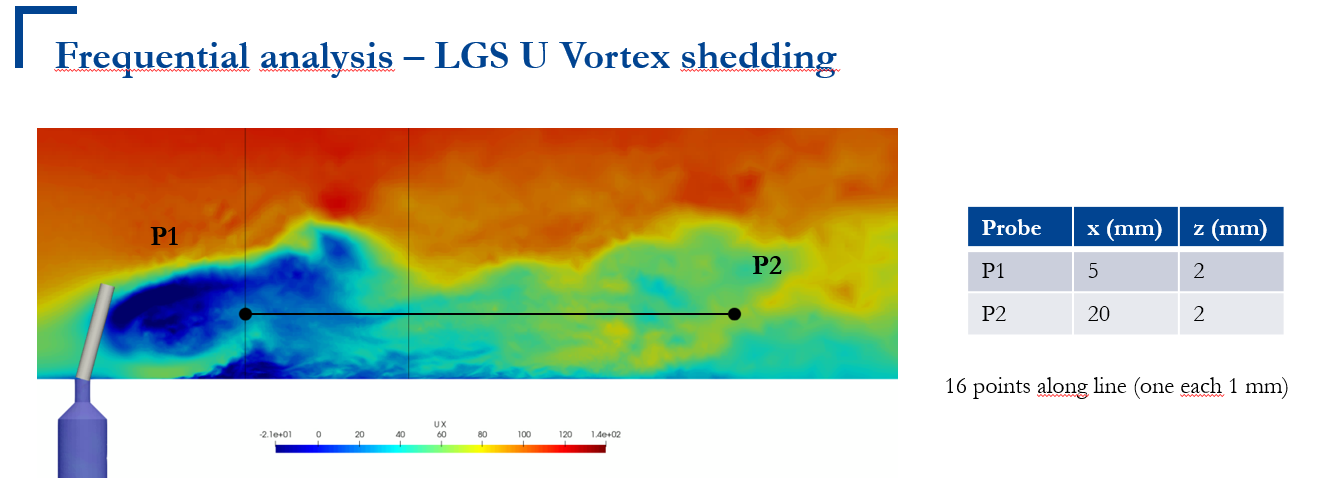
\includegraphics[scale=0.7]{./part2_developments/figures_ch6_lagrangian_JICF/probes_U_planey0}
	\caption{Probes for $U$ study}
	\label{fig:probes_U_planey0}
\end{figure}



\section{Conclusions}